\section{半精度、单精度与双精度运算}

大家好，在本文章中我将带大家了解GPU中的不同数据类型和大小。但在这里我想先告诉大家一点，理解数据类型和大小就像在工具箱
中选择合适的工具一样，这是高效且准确完成任务的基础。在GPU计算领域，与CPU类似，我们会根据需求采用不同的方式来存储数
值。例如我们先从整数开始，对于整数我们可以使用八位、16位、32位甚至64位，位数越多能存储的数值就越大。例如一个八位整
数在无符号的情况下可以存储0到255之间的值。如果是有符号变量，则范围为-127到128。

\subsection{整数与浮点类型}

对于64位整数，我们可以存储大得多的数值，最高可达约1800亿亿。这些数字也有不同的大小，当我们处理带小数点的数字时会使
用浮点表示法。例如我们有16位，这被称为半精度。然后是32位，这被称为单精度。最后是64位，这被称为双精度。

在C或 CUDA 编程语言中用int声明变量会使用32位。如果我们将int替换为long，那么通常在内存中会使用64位。
同样的另一方面，如果我们用float声明变量，则在内存中使用32位。但如果将float替换为double，则会在内存中使
用64位。
\subsection{半精度、单精度与双精度的差异}

半精度，它也被称为FP16。这是一种二进制浮点格式，在计算机内存中占用16位，即二个字节。这里的16指的是16位，FP指
的是浮点。半精度提供的数值精度较低，但所需的计算资源更少。

单精度也被称为 FP32。这里的32同样是指存储该类型变量所需的位数，FP指的是浮点。半精度适用于机器学习和图形处理等特
定应用，这些场景通常不需要高精度。这种类型在速度和精度之间取得了折衷，因此单精度成为各类计算任务的首选。

接下来是双精度或称FP64类型。这种类型被视为精度上的强力引擎。这是因为科学计算和复杂仿真中，每一个小数点都可能引发蝴蝶
效应。因此依赖这种类型依赖FP64精度。这种类型确保了对气候模式或分子结构等现象的仿真尽可能接近现实。这种设计及不同的精
度层级，使GPU能够灵活适应各种行业和应用场景。


\begin{figure}
    \centering
    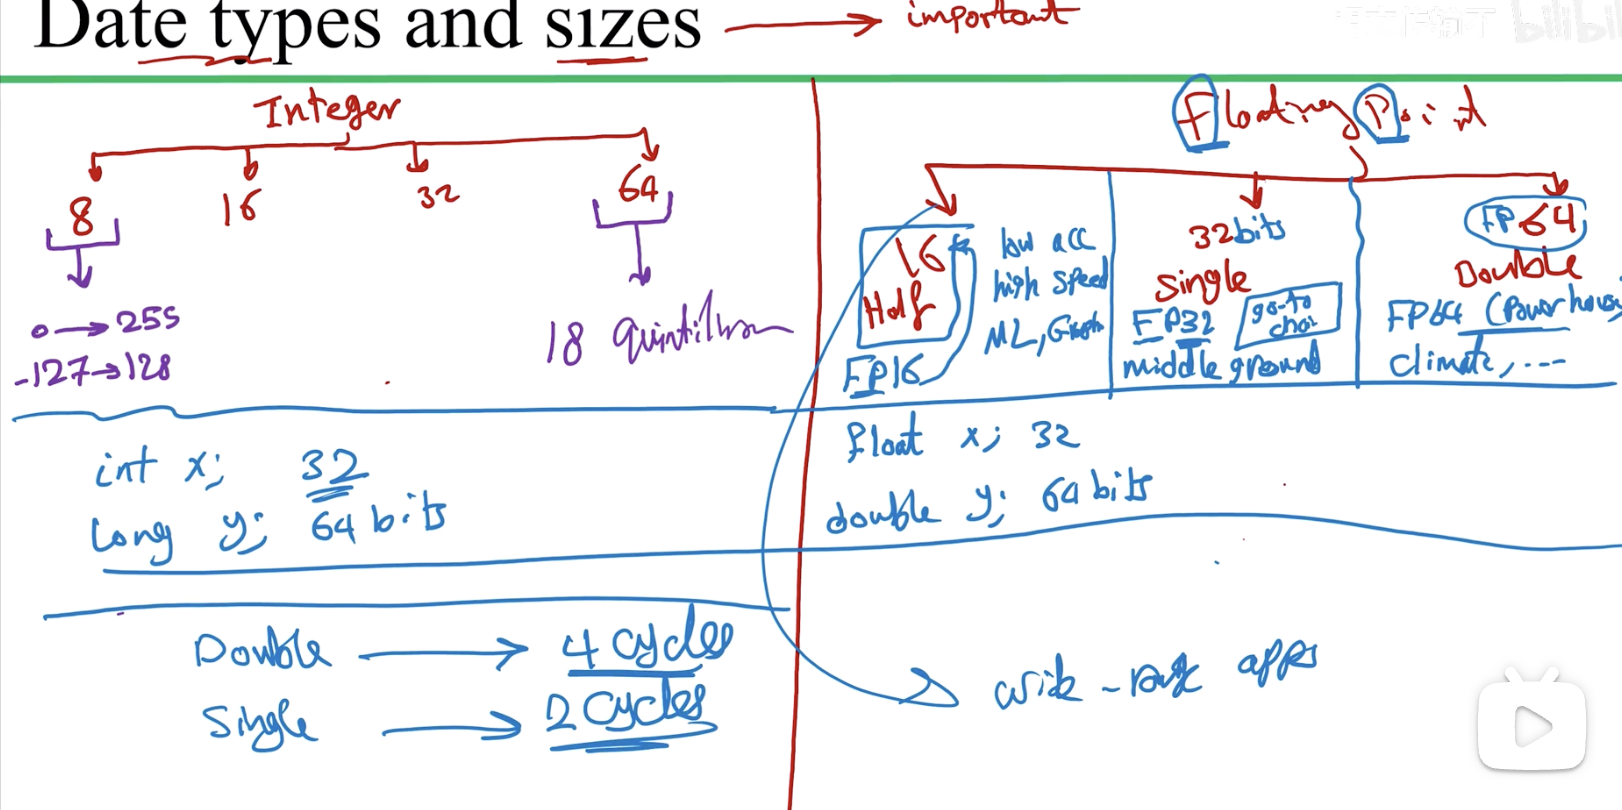
\includegraphics[width=0.75\linewidth]{resources/cuda-036.png}
    \caption{数据类型}
    \label{fig:placeholder}
\end{figure}


\subsection{PI的精度对比}

正因如此，在一篇研究不同GPU数据类型的论文中发现，双精度计算需要四个执行周期。而单精度计算仅需两个周期，这表明双精度虽
然更慢，但提供了更高的精度。例如，如果我们有这里的这段代码，比如floatX，Y和Z我们设X等于10.3。Y等于5.8，
并有一条指令或操作，其中Z等于X加Y那么此操作将仅需两个周期即可完成。然而如果我们将float类型替换为double，同
样的加法操作则需要四个周期才能完成。这种周期数的变化源于双精度数据类型更高的精度和处理需求。

\begin{figure}
    \centering
    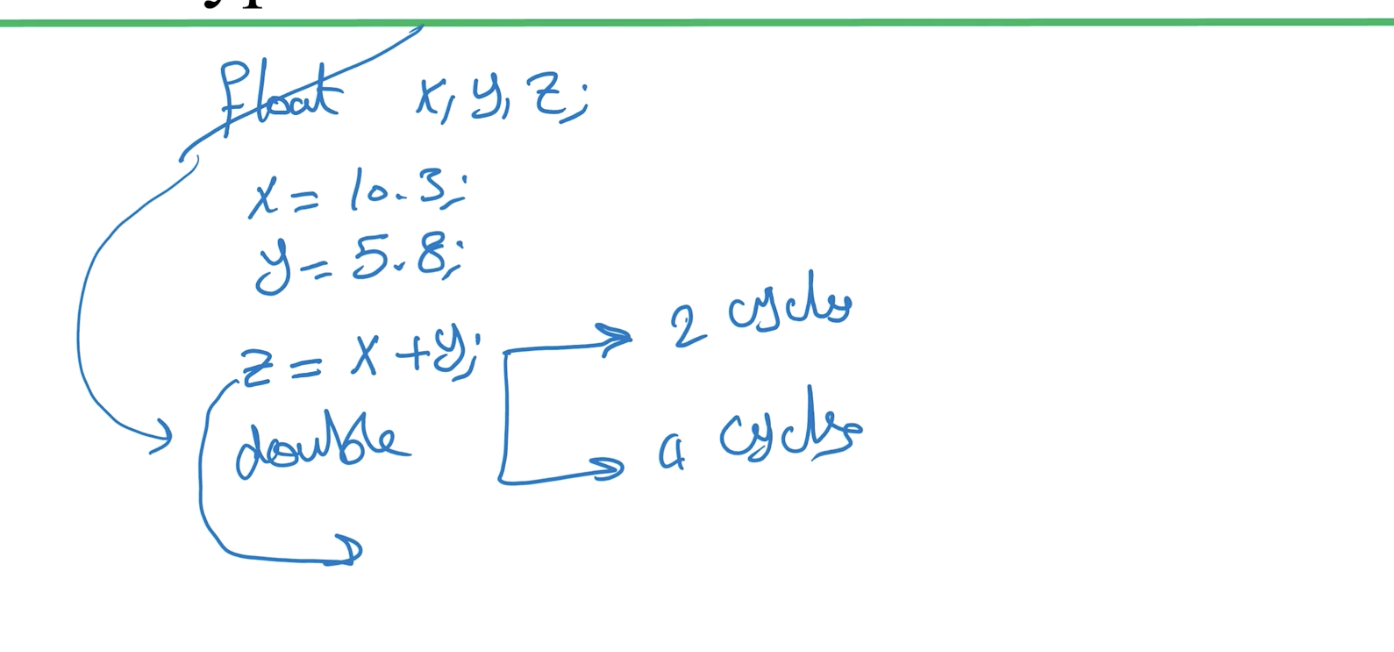
\includegraphics[width=0.75\linewidth]{resources/cuda-037.png}
    \caption{不同计算类型所需时钟周期}
    \label{fig:placeholder}
\end{figure}


为了更清楚的说明，让我们看看圆周率PI在不同浮点精度下的表示方式。在半精度格式中，PI仅保留小数点后两位数字，这意味着像
这样的小数值，正因如此，当需要高精度时会选择双精度。在单精度格式中，这一位数增加到7位，而在双精度格式中进一步扩展到15
位。它实际上会被近似为零。在此处所示的这个数值无法在半精度格式中被准确表示。这一限制是因为半精度最多只支持小数点后2到3
位数字。半精度不适合表示如此精细的数值。

\begin{figure}
    \centering
    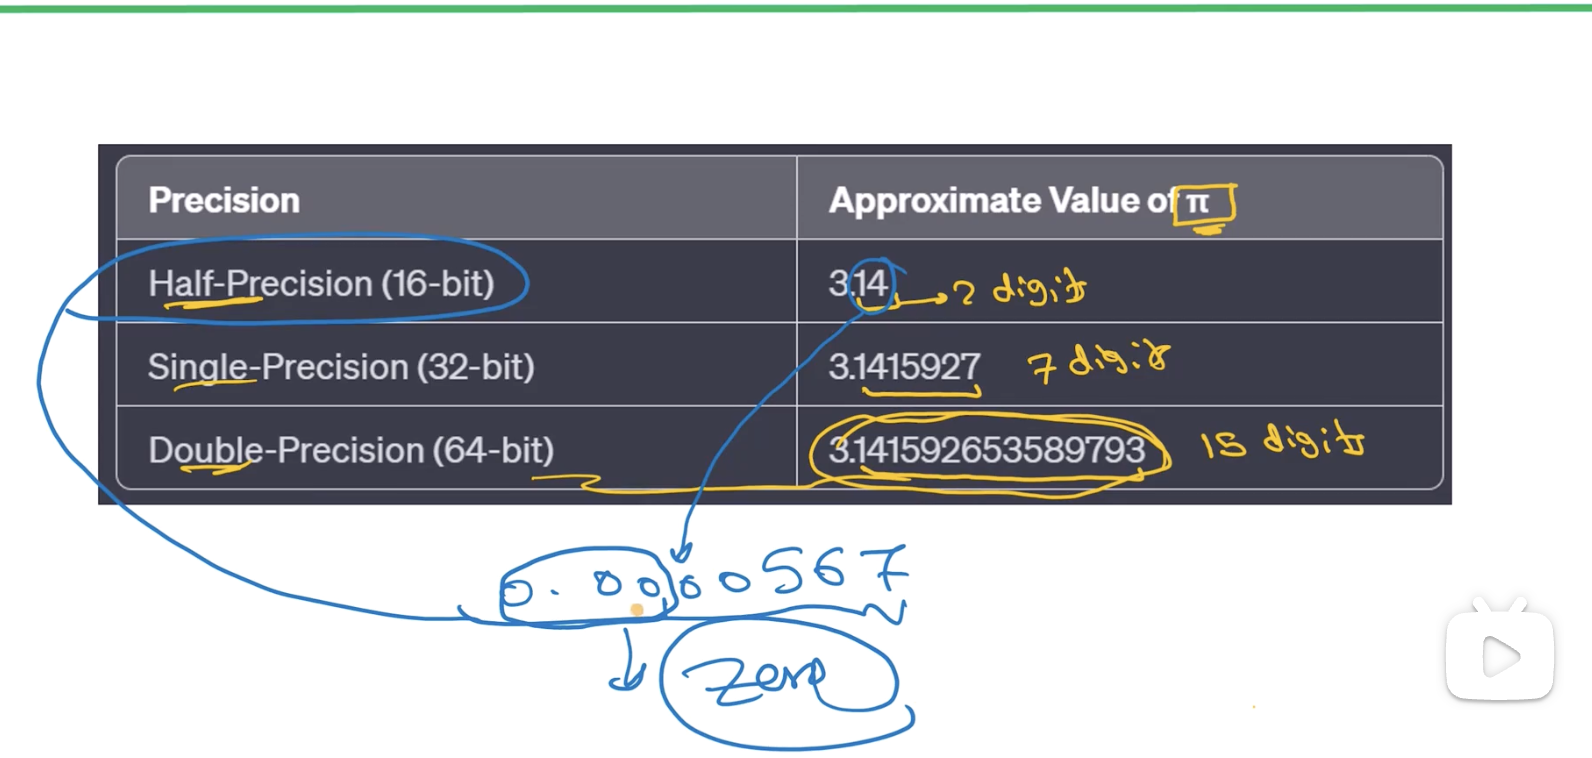
\includegraphics[width=0.75\linewidth]{resources/cuda-038.png}
    \caption{PI的精度}
    \label{fig:placeholder}
\end{figure}
